\documentclass{beamer}[11pt]

	\usepackage{ascii}
	\usepackage{fontspec}
	\usepackage[T1]{fontenc}
	\usepackage[french]{babel}
	\usepackage{graphicx}
	\usepackage{amsmath,amsfonts}
	\usepackage{mathrsfs}
	\usepackage{stmaryrd}
	\usepackage{verbatim}
	\usepackage{xcolor}

	\usepackage{color}
	\usepackage{listings}

	\renewcommand{\ttfamily}{\asciifamily}

	\lstset{
	  escapeinside={\%*}{*}, % Ce que vous mettrez entre %* et * dans le CODE sera compilé comme du LaTeX
	  language=Python,
	  basicstyle=\ttfamily\scriptsize,
	  tabsize=2,
	  breakatwhitespace=true,
	  breaklines=true,
	  showstringspaces=false,
	  showtabs=false,
	  numbers=left,
	  numbersep=5pt,
	  stepnumber=1,
	  keywordstyle=\color{purple},
	  identifierstyle=\color{blue},
	  stringstyle=\color[HTML]{008800},
	  commentstyle=\color[gray]{0.25},
	  numberstyle=\tiny\color{gray}
	}

	\geometry{paperwidth=160mm,paperheight=120mm}

	\title[Construction d'un réseau routier \hspace{2.5cm}\insertframenumber/\inserttotalframenumber]{Modélisation, construction d'un réseau routier}
	\author{Numéro 32203}
	\date{8 juin 2019}

	\newtheorem{thm}{Théorème}
	\newtheorem{déf}{Définition}
	\newtheorem{prop}{Propriété}
	\newtheorem{rem}{Remarque}

	\usetheme{Warsaw}

\begin{document}

  \begin{frame}
    \titlepage
  \end{frame}

  \begin{frame}
    \tableofcontents
  \end{frame}

	\section{Construction du graphe initial}

		\subsection{Cadre}

			\begin{frame}
				\frametitle{Cadre de l'étude}
				\begin{figure}[t]
					\centering
						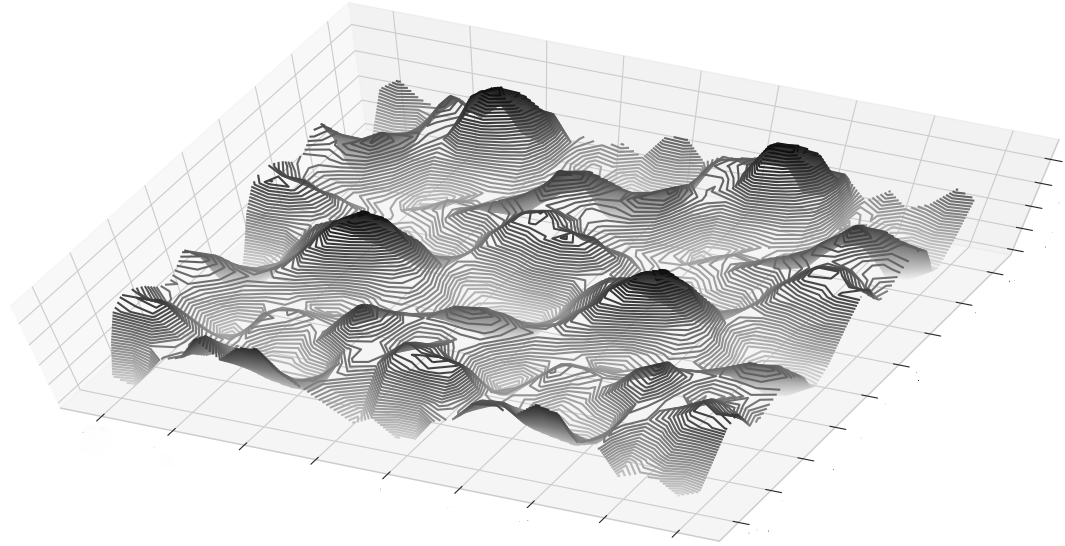
\includegraphics[width=1\textwidth]{Pics/img1.png}
				\end{figure}
			\end{frame}

		\subsection{Construction}

			\begin{frame}
				\frametitle{Construction par plus courts chemins}
				\begin{figure}[t]
					\centering
						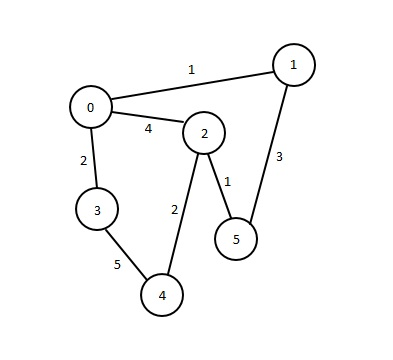
\includegraphics[width=0.5\textwidth]{Pics/grph.jpg}
				\end{figure}
			\end{frame}

			\begin{frame}
				\begin{figure}[t]
					\centering
						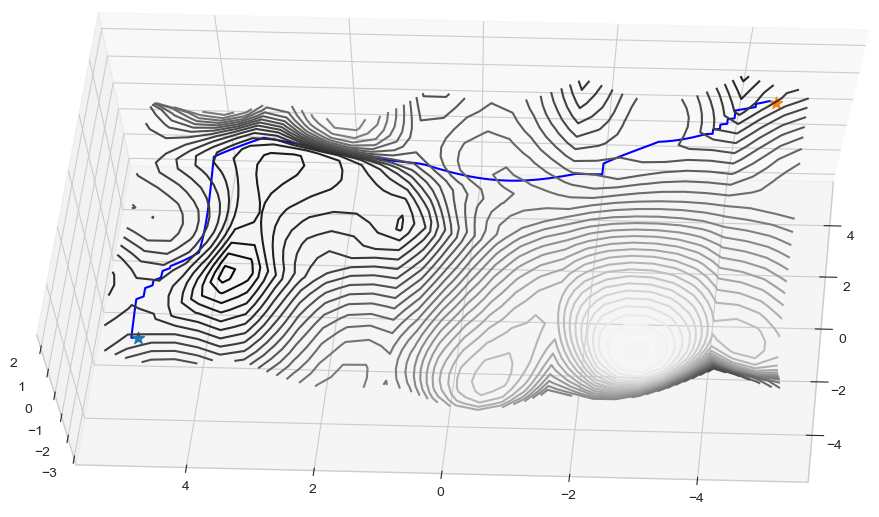
\includegraphics[width=1\textwidth]{Pics/lacets.png}
				\end{figure}
			\end{frame}

		\subsection{Jonctions}

			\begin{frame}
				\frametitle{Problème des jonctions}
				\begin{figure}[t]
					\centering
						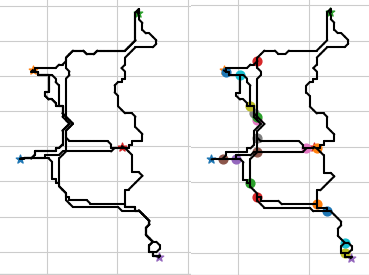
\includegraphics[width=.6\textwidth]{Pics/normcomp.png}
				\end{figure}
			\end{frame}

			\begin{frame}[fragile]
				\begin{verbatim}
Entree : N = (V,R) le graphe precedent
Pour r,s deux routes de R :
I = les sommets communs a r,s
  Tant que I n'est pas vide :
    Retirer un sommet v de I
    Si il s'agit d'une jonction :
      Raccorder r,s a la jonction
    Sinon:
      Creer une jonction en ce sommet
\end{verbatim}
			Il faut ensuite retirer les sommets vides, les boucles et routes en double éventuelles et mettre à jour la structure de données...
			\end{frame}

	\section{Coûts}

		\subsection{Coût de construction}

			\begin{frame}
				\frametitle{Principe}

				$$C_{c}(r) = \alpha L(r) + \beta V_{deplace}(r)$$

				\begin{figure}[t]
					\centering
						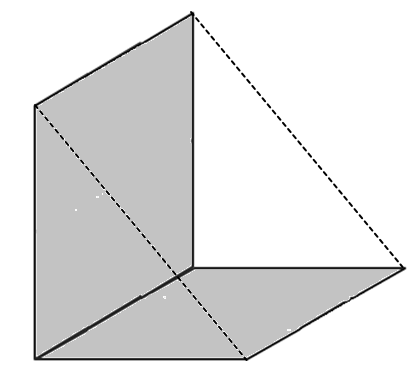
\includegraphics[width=0.5\textwidth]{Pics/Tunn.png}
				\end{figure}

			\end{frame}

		\subsection{Coût d'usage}

			\begin{frame}
				\frametitle{Modèle}

				$$C_{u,r} = \Delta E_{m} \times \Delta t$$

				$\Delta E_{m} = \Delta E_{c} + \Delta E_{p,grav} + E_{roulement} + E_{frott} = m g (1+c_{r}) \Delta z + S \rho v^{3} \Delta t$

				\begin{figure}[t]
					\centering
						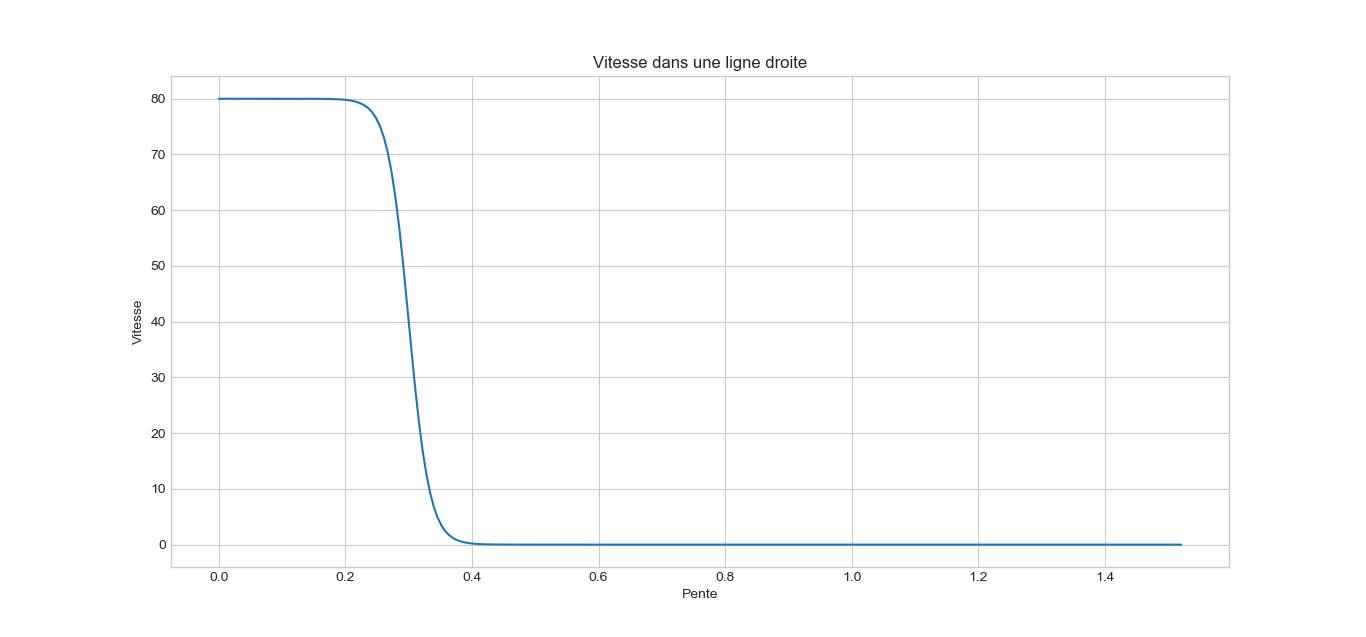
\includegraphics[width=0.9\textwidth]{Pics/vit.png}
				\end{figure}

			\end{frame}

			\begin{frame}
				\frametitle{Prise en compte des virages}

				$F_{ie} = m \Omega^{2} R$

				$\tan \alpha = \frac{F_{ie}}{mg} = \frac{v^{2}}{Rg}$

				Soit $$v < \sqrt{Rg \tan \alpha_{max}}$$

				\begin{figure}[t]
					\centering
						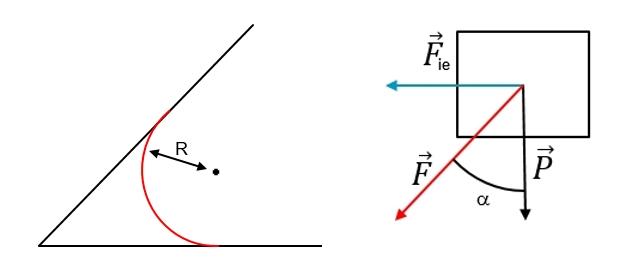
\includegraphics[width=0.8\textwidth]{Pics/forvir.jpg}
				\end{figure}
			\end{frame}

			\begin{frame}
				\frametitle{Synthèse}

				$$C_{u} = \sum_{i < j}{C_{u}(i,j)}$$
				$$C_{u}(i,j) = \int_{i \leftrightarrow j}{E(t)dt} = \sum_{r \in i \leftrightarrow j}{C_{u,r}} + C_{vir}$$

				\begin{figure}[t]
					\centering
						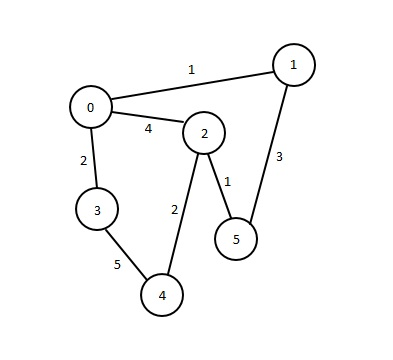
\includegraphics[width=0.4\textwidth]{Pics/grph.jpg}
						\caption{{0,1} est emprunté quatre fois : $0 \leftrightarrow 1, 0 \leftrightarrow 5, 3 \leftrightarrow 1, 3 \leftrightarrow 5$}
				\end{figure}
			\end{frame}

		\subsection{Un compromis}

			\begin{frame}
				\frametitle{Un compromis}

				$$ C = f(C_{c},C_{u})$$

				On cherche à minimiser C

				La fonction retenue est la moyenne géométrique

			\end{frame}

	\section{Optimisations}

		\subsection{Algorithmes déterministes}

			\begin{frame}[fragile]
				\frametitle{Suppression d'arcs inutiles}

\begin{verbatim}
Entree : N = (V,R)
Pour r une route de R :
  Si r ne fait pas partie d'un plus court chemin :
    Retirer r
\end{verbatim}

				Complexité : $ O(|R|^{2}) $

			\end{frame}

			\begin{frame}[fragile]
				\frametitle{Suppression des $K_{3}$}

\begin{verbatim}
Entree : N = (V,R)
Pour tout sous-graphe triangulaire de N :
  Si le plus long cote est assez grand devant les deux autres :
    Le retirer
\end{verbatim}

			On se donne un critère que l'on fait varier

			$x \in [0,1], (1+x) c_{c} c_{u} \leq (a_{c} + b_{c})(a_{u} + b_{u})$

			\begin{figure}[t]
				\centering
					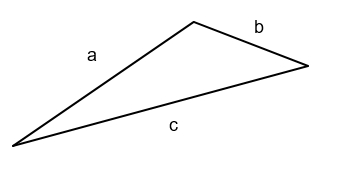
\includegraphics[width=0.4\textwidth]{Pics/tri.jpg}
			\end{figure}

			\end{frame}

		\subsection{Algorithme exhaustif}

			\begin{frame}[fragile]
				\frametitle{Recherche du minimum par backtracking}
\begin{verbatim}
Entree : N = (V,R)
Pour une route r de R :
  P = N prive de r
  Si C(P) < C(N) :
    N = P
\end{verbatim}

			Complexité : $O(|R|!)$, améliorable en $O(2^{|R|})$

			\end{frame}

		\subsection{Probabilisation}

			\begin{frame}
				\frametitle{Le recuit simulé}

				Principe : descente du gradient probabiliste

				Analogie thermodynamique : si deux états $E_{1},E_{2}$ sont distants d'une énergie $\Delta E$ à une température T, l'algorithme passe du premier au second si $\Delta E < 0$ avec probabilité 1 ou avec probabilité $\exp(\frac{\Delta E}{k_{B}T})$ sinon. T diminue durant l'exécution.

				Avantage : permet de s'extraire des minima locaux contrairement à la descente du gradient
				Inconvénient : ne converge que si T diminue peu rapidement

			\end{frame}

			\begin{frame}
				\frametitle{Probabilisation de l'algorithme}
\begin{verbatim}
Entree : N = (V,R)
Pour une route aleatoire r de R ne brisant pas la connexite :
  Diminuer T
  P = N prive de r
  Delta = C(P) - C(R)
  Si Delta < 0 ou random() < exp(Delta/T):
    N = P
\end{verbatim}
			Complexité : $O(|R|^{2})$ par tour de boucle
			\end{frame}

	\begin{frame}
		\frametitle{Conclusion}
		\begin{figure}[t]
			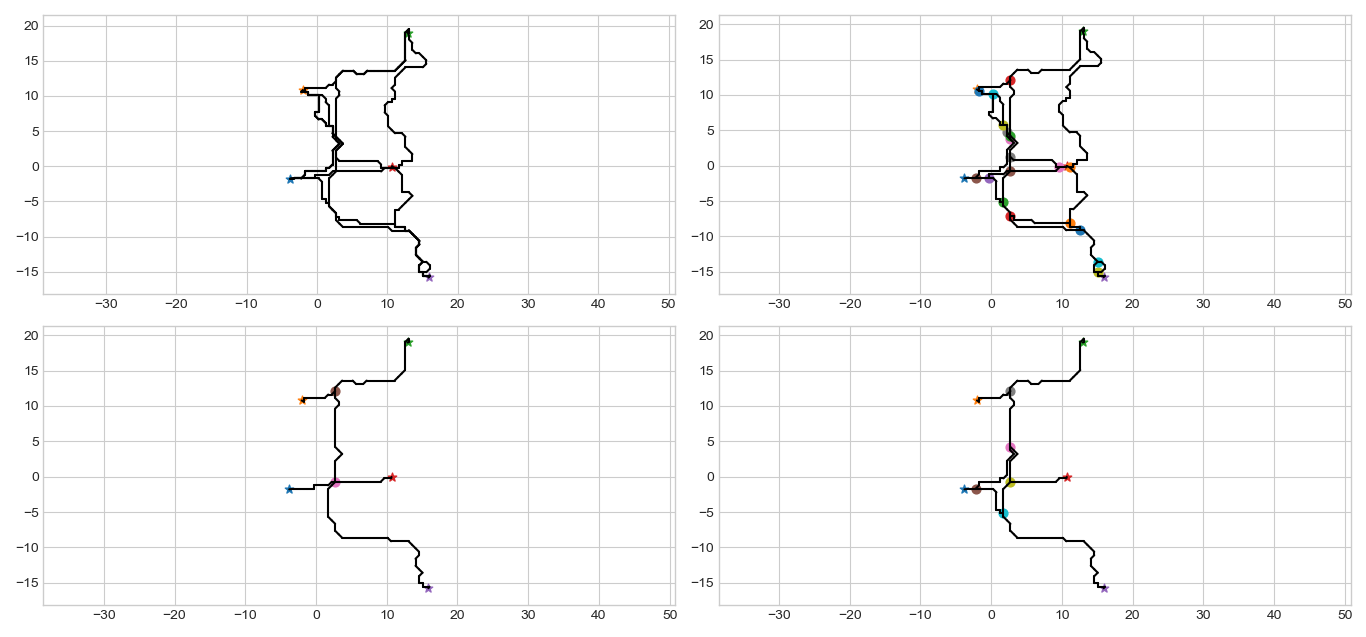
\includegraphics[width=1\textwidth]{Pics/g21.png}
		\end{figure}
	\end{frame}

	\begin{frame}
		\frametitle{Conclusion}
		\begin{figure}[t]
			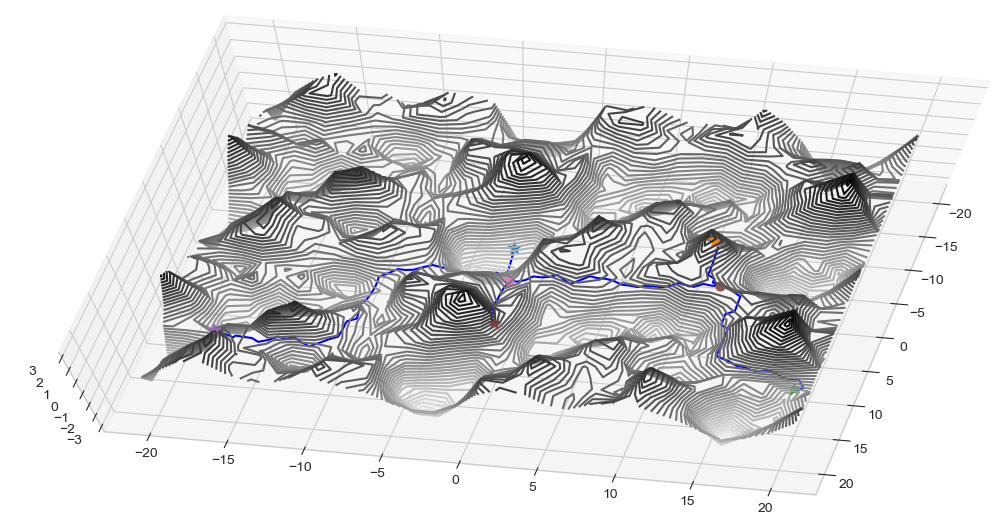
\includegraphics[width=1\textwidth]{Pics/g22.png}
		\end{figure}
	\end{frame}

	\begin{frame}
		\frametitle{Conclusion}
		\begin{figure}[t]
			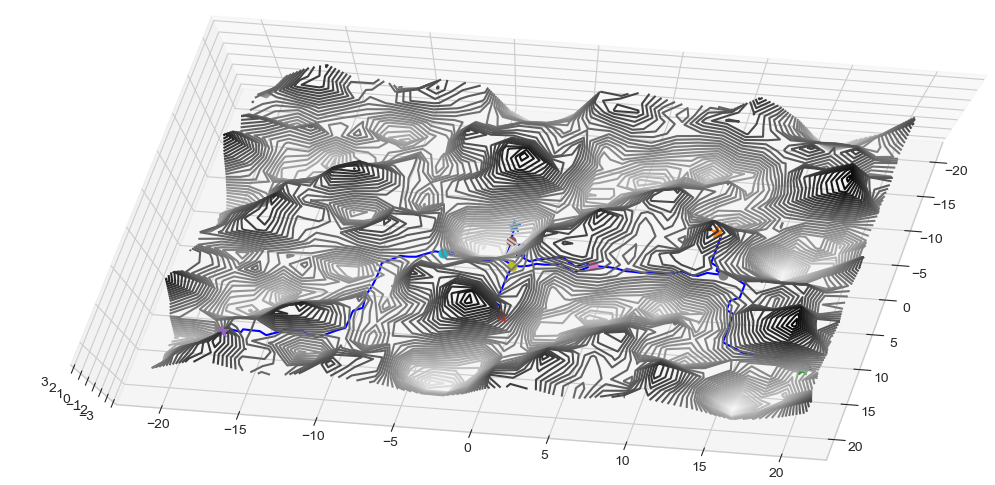
\includegraphics[width=1\textwidth]{Pics/g23.png}
		\end{figure}
	\end{frame}

\appendix

	\begin{frame}
		\tableofcontents
	\end{frame}

	\section{Galerie}

		\begin{frame}
			\begin{figure}[t]
				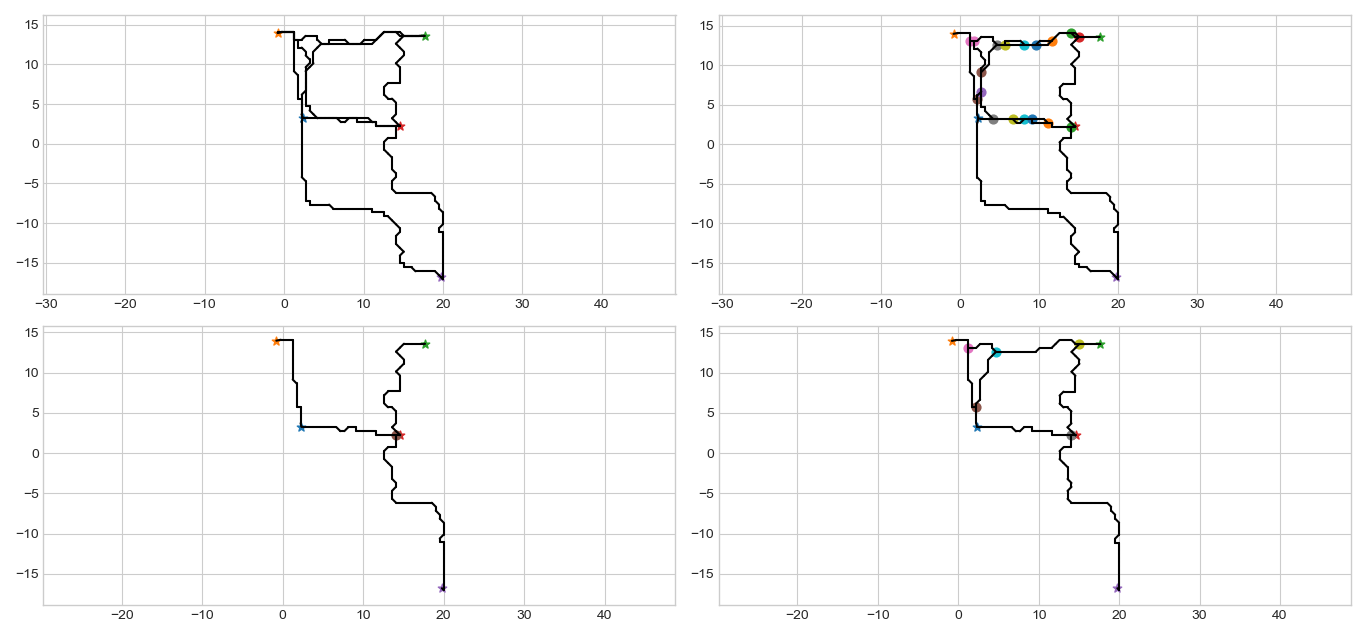
\includegraphics[width=1\textwidth]{Pics/g11.png}
			\end{figure}
		\end{frame}

		\begin{frame}
			\begin{figure}[t]
				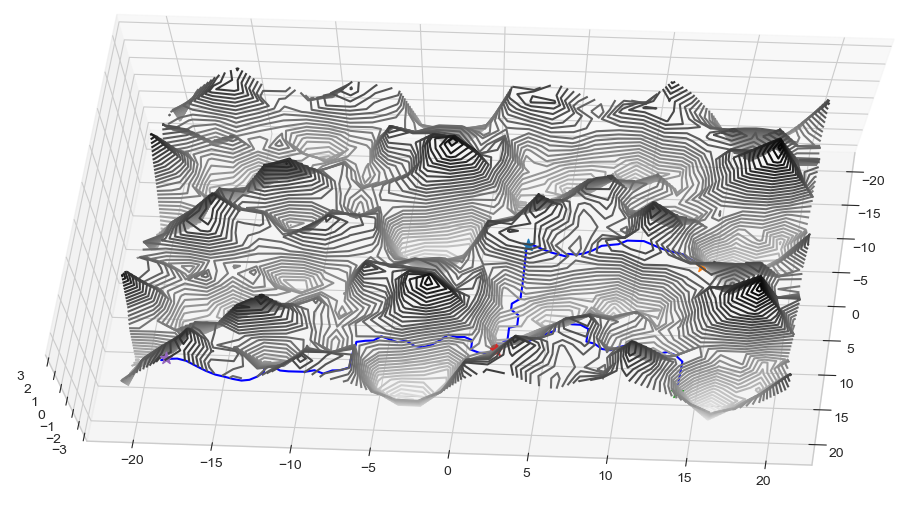
\includegraphics[width=1\textwidth]{Pics/g12.png}
			\end{figure}
		\end{frame}

		\begin{frame}
			\begin{figure}[t]
				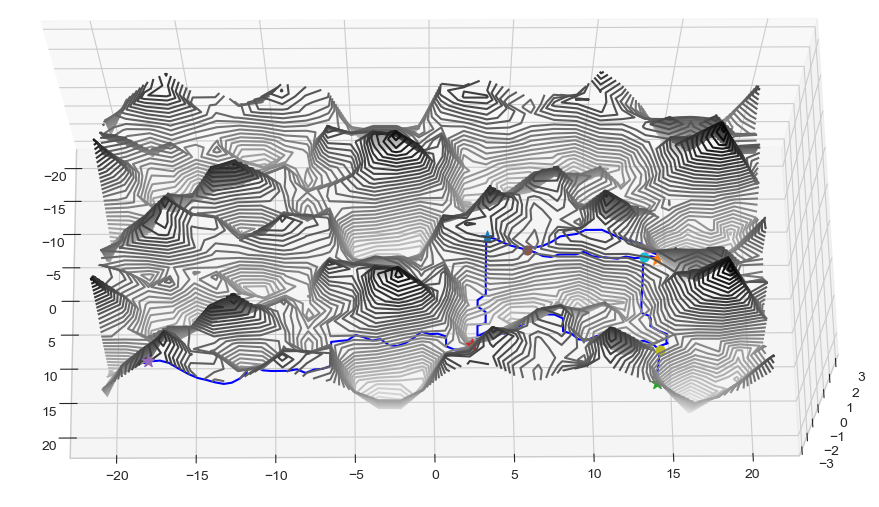
\includegraphics[width=1\textwidth]{Pics/g13.png}
			\end{figure}
		\end{frame}

		\begin{frame}
			\begin{figure}[t]
				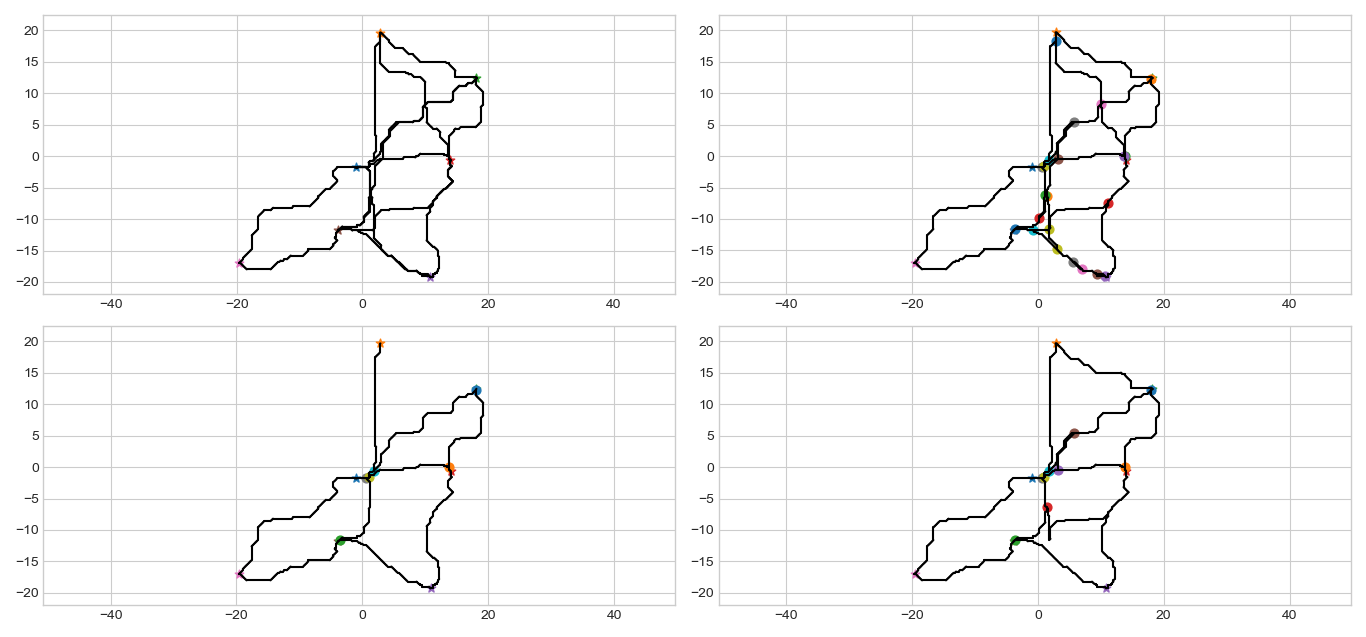
\includegraphics[width=1\textwidth]{Pics/g31.png}
			\end{figure}
		\end{frame}

		\begin{frame}
			\begin{figure}[t]
				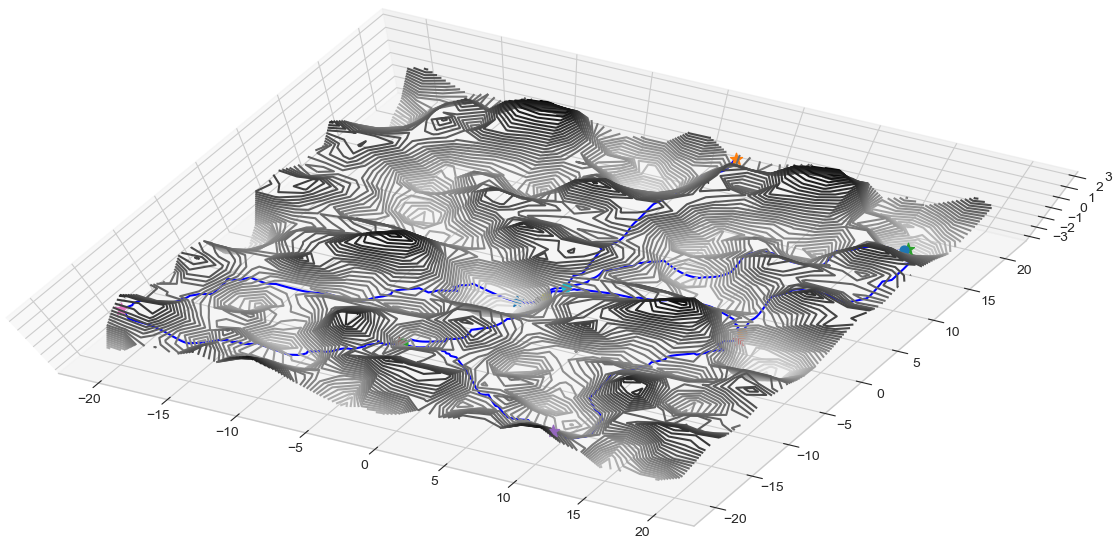
\includegraphics[width=1\textwidth]{Pics/g32.png}
			\end{figure}
		\end{frame}

		\begin{frame}
			\begin{figure}[t]
				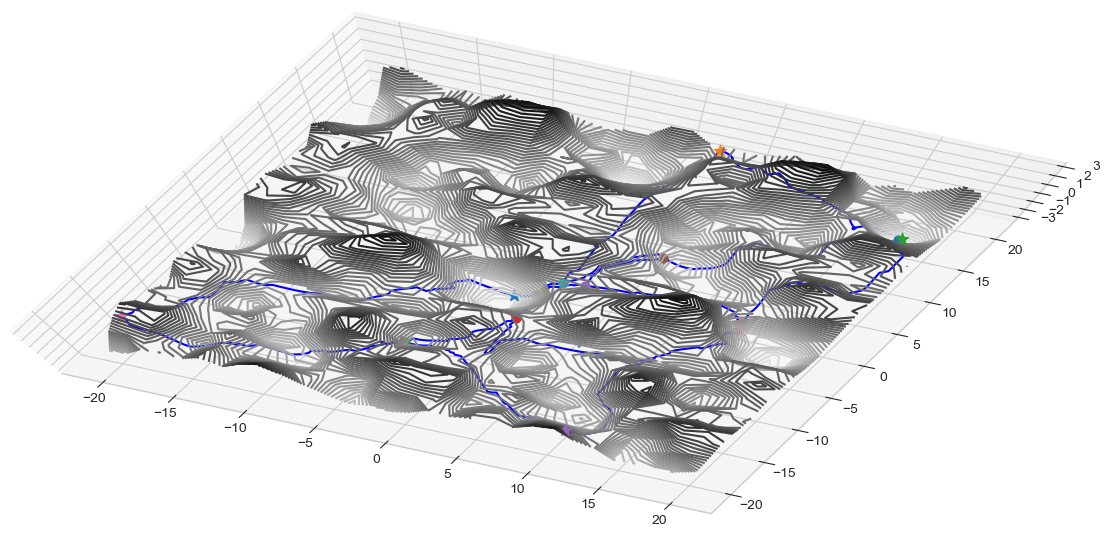
\includegraphics[width=1\textwidth]{Pics/g33.png}
			\end{figure}
		\end{frame}

	\section{Algorithmes}

		\begin{frame}[containsverbatim]
\begin{lstlisting}
import numpy as np
import matplotlib.pyplot as plt
from time import time
from copy import deepcopy
plt.style.use('seaborn-whitegrid')
from mpl_toolkits import mplot3d

carte = [4, 3, 2, 0, 1, 4, 1, 0, 2, 1, 3, 0, 0, 3, 0, 4, 0, 1, 4, 1, 0, 2, 3, 4]

def f(x,y,tab=carte) :
    '''Fonction donnant l'altitude d'un point de coordonnees (x,y)'''
    x /= 3
    y /= 3
    return (np.sin(x-y+tab[0]) ** tab[1] + np.sin(y * tab[2]) * np.cos(x-tab[3]) + tab[4] * np.cos(tab[5]*y-tab[6]) ** tab[7]  + np.sin(np.cos(x) * y)/tab[8] - tab[9] * np.sin(x+tab[10]) ** tab[11] + np.sin(x) * np.cos(y-tab[12]) + tab[13] * np.cos(tab[14]*y+tab[15]) ** 2) - (abs(np.sin(-x-y+tab[16]) ** tab[17]) + abs(np.sin(y * tab[18]-1)) * abs(np.cos(x+tab[19])) + abs(tab[20] * np.cos(tab[21]*x+tab[22]) ** tab[23]))
\end{lstlisting}
		\end{frame}

		\begin{frame}[containsverbatim]
			\frametitle{Discrétisation}

\begin{lstlisting}
def discretise(f,s0,sf,h) :		# Complexite : quadratique en la resolution
    (x0,y0) = s0
    (xf,yf) = sf
    n = int(abs(xf-x0) // h) + 1
    p = int(abs(yf-y0) // h) + 1
    h = 0.5 * (abs(xf-x0) / n + abs(yf-y0) / p)
    n += 1
    p += 1
    S = [(x0+i*h,y0+j*h,f(x0+i*h,y0+j*h)) for i in range(n) for j in range(p)]
    A = [[] for i in range(n) for j in range(p)]

    for x in range(n*p) :
        for a in [-1,0,1] :
            for b in [-1,0,1] :
                jx,ix = divmod(x,n)
                y = a + ix + n * (b + jx)
                if y != x and 0 <= a + ix < n and 0 <= b + jx < p :
                    c = cout_construction([S[x],S[y]])
                    A[y].append((x,c))
                    A[x].append((y,c))
    return S,A,n,p,h
\end{lstlisting}
		\end{frame}

% %*\hyperlink{disc2}{\beamergotobutton{[\dots]}}*
% %*\hyperlink{disc1}{\beamerreturnbutton{[\dots]}}*

		\begin{frame}[containsverbatim]
\begin{lstlisting}
class Heap :		# Structure de tas binaire

  def tasse(self,i) :
      n = len(self.heap) - 1
      if 2 * i + 1 >= n :
          self.percole(i)
      else :
          self.tasse(2*i)
          self.tasse(2*i+1)
          self.percole(i)

  def __init__(self,l=[],compare=lambda a,b:a<b) :
      self.heap = [len(l)] + l
      self.comp = compare
      self.tasse(1)

  def remonte(self,i) :
      if i // 2 > 0 :
          if self.comp(self.heap[i],self.heap[i//2]) :
              self.heap[i],self.heap[i//2] = self.heap[i//2],self.heap[i]
              self.remonte(i//2)
\end{lstlisting}
		\end{frame}

		\begin{frame}[containsverbatim]
\begin{lstlisting}[basicstyle=\tiny]

	def add(self,x) :
			self.heap.append(x)
			self.heap[0] += 1
			self.remonte(self.heap[0])

	def take(self) :
			self.heap[0] -= 1
			x = self.heap.pop()
			return x

	def percole(self,i) :
			if 2 * i + 1 >= len(self.heap) - 1 :
					if 2 * i < len(self.heap) - 1 :
							j = 2 * i
							if self.comp(self.heap[j],self.heap[i]) :
									self.heap[i],self.heap[j] = self.heap[j],self.heap[i]
									self.percole(j)
			else :
					if self.comp(self.heap[2*i],self.heap[2*i+1]) :
							j = 2 * i
					else :
							j = 2 * i + 1
					if self.comp(self.heap[j],self.heap[i]) :
							self.heap[i],self.heap[j] = self.heap[j],self.heap[i]
							self.percole(j)

	def take_min(self) :
			self.heap[1],self.heap[-1] = self.heap[-1],self.heap[1]
			x = self.take()
			self.percole(1)
			self.heap[0] -= 1
			return x
\end{lstlisting}
		\end{frame}

		\begin{frame}[containsverbatim]
			\frametitle{Algorithme de Dijkstra}
\begin{lstlisting}
def dijkstra(S,A,n,p,h,s0,sf) :		# Complexite : O(|R|log|V|)
    deb = pos(s0,S,h)
    fin = pos(sf,S,h)
    pred = [-1 for _ in S]
    dist = [np.infty for _ in S]
    dist[fin] = 0
    pq = Heap([(0,fin)],lambda a,b : a[0] < b[0])
    deja_vu = [False for s in S]

    while len(pq.heap) > 1 :
        u = pq.take_min()[1]
        if deja_vu[u] :
            continue
        deja_vu[u] = True
        for v,w in A[u] :
            if dist[v] > dist[u] + w :
                dist[v] = dist[u] + w
                pred[v] = u
                pq.add((dist[v],v))

    C = [s0]
    s = deb
    while s != fin :
        C.append(S[s])
        s = pred[s]
    C.append(sf)
    return C
\end{lstlisting}
		\end{frame}

		\begin{frame}[containsverbatim]
\begin{lstlisting}[basicstyle=\tiny]
class Map :		# Structure comprenant les elements essentiels de la modelisation

		def __init__(self,pt,s0=(-20,-20),sf=(20,20),h=0.5,graph=-1,dmin = 30,cc=-1,cu=-1) :
				if graph  == -1 :
						(S,A,n,p,h) = discretise(f,s0,sf,h)
						self.graph = (S,A,n,p,h,s0,sf)
				else :
						self.graph = graph
				self.network = []
				self.towns = pt
				self.cc = cc
				self.cu = cu

				self.init()

    def init(self,dmin=30) :		# Construit le graphe initial par plus courts chemins
        l = len(self.towns)
        (S,A,n,p,h,s0,sf) = self.graph

        for i in range(l) :
            t = Node(self.towns[i],tow=True,nb = i)
            self.network.append(t)
            self.network[i].roads = []

        ct = 0
        for i in range(l) :
            for j in range(i + 1, l) :
                if abs(self.towns[i][0] - self.towns[j][0]) < dmin and abs(self.towns[i][1] - self.towns[j][1]) < dmin :
                    ct += 1
                    C = dijkstra(S,A,n,p,h,self.towns[i],self.towns[j])
                    r = Road(i,j,C,False)
                    self.network[i].roads += [r]
                    self.network[j].roads += [r.retourne()]
\end{lstlisting}
		\end{frame}

		\begin{frame}[containsverbatim]
\begin{lstlisting}
def __repr__(self) :		# Outil de trace permettant de visualiser le reseau en 2D
		N = self.network
		for s in N :
				(x,y,z) = s.coord
				for r in s.roads :
						if len(N) > r.end > s.id :
								u = N[r.end]
								(x2,y2,z2) = u.coord
								if r.tunn :
										for i in range(len(r.path) - 1) :
												(x1,y1,z1) = r.path[i]
												(x2,y2,z2) = r.path[i+1]
												plt.plot([x1,x2],[y1,y2],'--',color='black')
								else :
										for i in range(len(r.path) - 1) :
												(x1,y1,z1) = r.path[i]
												(x2,y2,z2) = r.path[i+1]
												plt.plot([x1,x2],[y1,y2],color='black')
				if s.town :
						plt.scatter(x,y,marker='*',s=40)
				elif len(s.roads) > 2 :
						plt.scatter(x,y,s=40)
		plt.axis('equal')
		plt.grid()
		return ""
\end{lstlisting}
		\end{frame}

		\begin{frame}[containsverbatim]
\begin{lstlisting}[basicstyle=\tiny]
def plot_3D(self) :			# Outil de trace permettant de visualiser le reseau en 3D
		N = self.network

		(x0,y0,z0) = self.graph[0][0]
		(xf,yf,zf) = self.graph[0][-1]

		x = np.linspace(x0, xf, 30)
		y = np.linspace(y0, yf, 30)

		X, Y = np.meshgrid(x, y)
		Z = np.vectorize(f)(X, Y)

		fig = plt.figure()
		ax = plt.axes(projection='3d')
		ax.contour3D(X, Y, Z, 50, cmap='binary')

		for i in range(len(N)) :
				if len(N[i].roads) > 0 :
						(xi,yi,zi) = N[i].coord
						if N[i].town :
								ax.scatter(xi,yi,zi,marker='*',s=80)
						elif len(N[i].roads) > 2 :
								ax.scatter(xi,yi,zi,s=40)
						for r in N[i].roads :
								j = r.end
								if i < j :
										C = r.path
										xs = [c[0] for c in C]
										ys = [c[1] for c in C]
										zs = [c[2] for c in C]
										ax.plot3D(xs,ys,zs,color='b')
		plt.show()
\end{lstlisting}
		\end{frame}

		\begin{frame}[containsverbatim]
\begin{lstlisting}
def copy(self) :				# Complexite : O(|V|)
		P = []
		pt = self.towns

		for s in self.network :
				t = Node(s.coord,[],s.town,s.id)
				P.append(t)

		for i in range(len(self.network)) :
				for r in self.network[i].roads :
						P[i].roads.append(Road(r.start,r.end,r.path,r.tunn,r.length,r.cc,r.cu,r.flux))

		M = Map(pt,graph=self.graph)
		M.network = P
		M.cc,M.cu = self.cc,self.cu
		return M
\end{lstlisting}
		\end{frame}

		\begin{frame}[containsverbatim]
\begin{lstlisting}
def normalize(self) :		# Complexite : au plus en O(r^2 |R|^5)
		cree_jonctions(self)
		fusion(self.network)    #Fusion des tronçons
		tailladeur(self.network)    #Suppression des premiers sommets vides
		supprime_nuls(self.network)     #Suppression des boucles
		supprime_doubles(self.network)  #Suppression des routes en double
		P = maj_indices(self.network)
		tailladeur(P)   #Suppression des derniers vides
		self.network = P
		self.update_fl()    #Mise a jour des coûts

def update_fl(self) :		# Complexite : O(|R|^2)
			for s in self.network :
					for r in s.roads :
							r.flux = 0
			self.cc,self.cu = attr_flux(self)

def longueur(L) :
    return sum([distance(L[i],L[i+1]) for i in range(len(L) - 1)])
\end{lstlisting}
		\end{frame}

		\begin{frame}[containsverbatim]
\begin{lstlisting}

def jonct(r1,r2) :			# Complexite : O(|c1||c2|)
    c1 = r1.path
    c2 = r2.path
    J = []
    for j in range(len(c2)) :
        for i in range(len(c1)) :
            if c1[i] == c2[j] :
                J.append(c1[i])

    return J

def attr_flux(N) :			# Complexite : O(|R|^2)
    G = [dijkstra_generalise(N.network,i) for i in range(len(N.network))]
    n = len(N.towns)
    cu = 0
    cc = 0
    for s in N.network :
        for r in s.roads :
            cc += r.cc
            r.flux = len([1 for (i,j) in [(i,j) for i in range(n) for j in range(n)] if r in G[i][j] + G[j][i]])
            cu += sum([r.cu for (i,j) in [(i,j) for i in range(n) for j in range(n)] if r in G[i][j] + G[j][i]])
    return cc,cu
\end{lstlisting}
		\end{frame}

		\begin{frame}[containsverbatim]
\begin{lstlisting}
def supprime_nuls(N) :	# Complexite : O(|R|)
    for s in N :
        for r in s.roads :
            if r.start == r.end or r.length == 0 :
                s.roads.remove(r)

def supprime_doubles(N) :	# Complexite : O(|R|)
    for s in N :
        D = []
        for r in s.roads :
            if r.end not in D :
                D.append(r.end)
        E = [np.infty for d in D]
        R = [0 for d in D]
        for i in range(len(R)) :
            for r in s.roads :
                if r.end == D[i] :
                    R[i] = r
                    break
            E[i] = r.cu
            for r in s.roads :
                if r.end == D[i] and r.cu < E[i] :
                    R[i] = r
                    E[i] = r.cu
        s.roads = R
\end{lstlisting}
		\end{frame}

		\begin{frame}[containsverbatim]
\begin{lstlisting}
def tailladeur(N) :		# Complexite : O(|V||R|)
    i = 0
    while i < len(N) - 1 :
        i += 1
        s = N[i]
        if not s.town and len(s.roads) == 1 :
            for r in s.roads :
                u = N[r.end]
                u.rem(s)
            s.roads = []
            i = 0
\end{lstlisting}
		\end{frame}

		\begin{frame}[containsverbatim]
\begin{lstlisting}
def cree_jonctions(M) : 	# Complexite : O(r^2 |V|^5)
    h = M.graph[4]
    for s in M.network :
        for u in M.network :
            if s.id < u.id :
                for rs in s.roads :
                    t = M.network[rs.end]
                    for ru in u.roads :
                        v = M.network[ru.end]
                        L = jonct(rs,ru)

                        while L != [] :
                            (x,y,z) = L.pop()
                            b = False

                            for w in M.network :
                                (xw,yw,zw) = w.coord
                                if 0.001 < abs(xw-x) < h/2 and 0.001 < abs(yw-y) < h/2 :
                                    b = True
                                    normalise_jonction(M.network,w,True)
                                elif abs(xw-x) < h/2 and abs(yw-y) < h/2 :
                                    b = True
                                    normalise_jonction(M.network,w)

                            if not b :
                                w = Node((x,y,z),tow=False,nb = len(M.network))
                                M.network.append(w)
                                normalise_jonction(M.network,w)
\end{lstlisting}
		\end{frame}

		\begin{frame}[containsverbatim]
\begin{lstlisting}
def normalise_jonction(N,t,existait=False) : 		# Complexite : O(|V||R|)
    for s in N :
        for r in s.roads :
            C = r.path
            u = N[r.end]
            for i in range(1, len(C) - 1) :
                if C[i] == t.coord :
                    s.rem(u)
                    u.rem(s)
                    cst = C[:i + 1]
                    ctu = C[i:]

                    if existait :
                        cst.append(t.coord)
                        ctu = [t.coord] + ctu

                    rst = Road(s.id,t.id,cst,traffic=r.flux)
                    rtu = Road(t.id,u.id,ctu,traffic=r.flux)
                    rts = rst.retourne()
                    rut = rtu.retourne()

                    s.roads.append(rst)
                    t.roads += [rts,rtu]
                    u.roads.append(rut)
\end{lstlisting}
		\end{frame}

		\begin{frame}[containsverbatim]
\begin{lstlisting}
def fusion(N) :		# Complexite : O(|R|)
    for s in N :
        r = s.roads
        if len(r) == 2 and not s.town :
            [rt,ru] = r
            t = N[rt.end]
            u = N[ru.end]
            cts = rt.path[::-1]
            csu = ru.path

            if cts[-1] == csu[0] :
                cts.pop()

            ctu = cts + csu

            t.rem(s)
            u.rem(s)
            s.roads = []
            rtu = Road(t.id,u.id,ctu)
            rut = rtu.retourne()
            t.roads.append(rtu)
            u.roads.append(rut)
\end{lstlisting}
		\end{frame}

		\begin{frame}[containsverbatim]
\begin{lstlisting}
def maj_indices(N) :	# Complexite : O(|R|^2)
    P = []
    i = 0
    j = 0
    for s in self.network :     #Mise a jour des indices
        if s.roads == [] :
            j += 1
        else :
            s.id = i
            for u in self.network :
                for r in u.roads :
                    if r.start == j :
                        r.start = i
                    if r.end == j :
                        r.end = i
            for u in P :
                for r in u.roads :
                    if r.start == j :
                        r.start = i
                    if r.end == j :
                        r.end = i
            P.append(s)
            i += 1
            j += 1
    for s in P :
        for r in s.roads :
            if r.end >= len(P) :
                s.roads.remove(r)
\end{lstlisting}
		\end{frame}

		\begin{frame}[containsverbatim]
\begin{lstlisting}
class Node :	# Structure representant les sommets du graphe

    def __init__(self,coordinates=(0.5,0.5,0),roads=[],tow=False,nb=-1) :
        self.coord = coordinates
        self.roads = []
        self.town = tow
        self.id = nb

    def rem(self,v) :
        for r in self.roads :
            if r.end == v.id :
                self.roads.remove(r)

    def __repr__(self) :
        (x1,y1,z1) = self.coord
        x = round(x1,3)
        y = round(y1,3)
        z = round(z1,3)
        if self.town :
            aff ="Ville localisee en {}".format((x,y,z))
        else :
            aff = "Jonction localise en {}".format((x,y,z))
        return aff
\end{lstlisting}
		\end{frame}

		\begin{frame}[containsverbatim]
\begin{lstlisting}
class Road :	# Structure representant les arêtes du graphe

    def __init__(self,start,end,path,is_tunnel=False,length=-1,cc=-1,cu=-1,traffic=0,i=1):
        self.start = start
        self.end = end
        self.path = path
        self.flux = traffic
        if length == -1 :
            self.length = longueur(path)
        else :
            self.length = length
        self.tunn = is_tunnel
        if cc == -1 :
            self.cc = cout_construction(path)
        else :
            self.cc = cc
        if cu == -1 :
            self.cu = cout_usage(path,6)
        else :
            self.cu = cu

    def retourne(self) :
        return Road(self.end,self.start,self.path[::-1],self.tunn,self.length,self.cc,self.cu,self.flux)
\end{lstlisting}
		\end{frame}

		\begin{frame}[containsverbatim]
\begin{lstlisting}
def cout_construction(C,i=1) :	# Complexite : O(|C|)
    S = 0
    delta = 10
    for i in range(len(C)-1) :
        dz = abs(C[i+1][2] - C[i][2])
        d = distance(C[i],C[i+1])
        S += delta * (d + dz * 1 * 0.5 * 36 * d ** 2)
    return S

def pente(i,j) :
    (xi,yi,zi),(xj,yj,zj) = i,j
    d = np.sqrt((xj-xi)**2 + (yj-yi)**2 + (zj-zi)**2)

    if xj == xi :
        if yj == yi :
            p = 0
        else :
            p = abs((zj-zi)/(yj-yi))
    else :
        if yj == yi :
            p = abs((zj-zi)/(xj-xi))
        else :
            p = abs((zj-zi)/(xj-xi) + (zj-zi)/(yj-yi))
    return p
\end{lstlisting}
		\end{frame}

		\begin{frame}[containsverbatim]
\begin{lstlisting}
def rayon(angle,l) :
    R = 0
    if abs(angle - 135) < 0.01 :
        R = 16 * l
    if abs(angle - 90) < 0.01 :
        R = 4 * l
    if abs(angle - 45) < 0.01 :
        R = l
    return R

def distance(i,j,k=1) :
    (xi,yi,zi),(xj,yj,zj) = i,j
    return ((xj-xi)**2 + (yj-yi)**2 + (zj-zi)**2) ** 0.5

def angle(a,b,c) :
    (xa,ya,za) = a
    (xb,yb,zb) = b
    (xc,yc,zc) = c
    u = (xa-xb,ya-yb)
    v = (xc-xb,yc-yb)
    q = (u[0] * v[0] + u[1] * v[1]) / np.sqrt(u[0] ** 2 + u[1] ** 2) / np.sqrt(v[0] ** 2 + v[1] ** 2)
    return np.arccos(round(q,5))
\end{lstlisting}
		\end{frame}

		\begin{frame}[containsverbatim]
\begin{lstlisting}[basicstyle=\tiny]
def cout_usage(C,l,i=1) :
    S = 0
    acc = 1
    alpha = np.tan(np.pi/14)
    g = 9.81
    cr = 0.01
    m = 2000
    ro = 1.3
    Sp = 4
    if len(C) < 3 :
        [a,b] = C
        dz = a[2] - b[2]
        p = pente(a,b)
        vmax = 80/(1 + np.exp(60 * p - 18)) / 3.6 + 1
        t = distance(a,b,i) / vmax
        Epp = m * (1 + cr) * g * dz
        Er = 0.5 * m * vmax ** 2
        Et = Sp * ro * vmax ** 3 * t
        if Epp + Et < 0 :
            S += 0
        else :
            S += t * (Er + Epp + Et)
    else :
        for i in range(len(C) - 2) :
            a = C[i]
            b = C[i+1]
            c = C[i+2]
            dz = C[i+1][2] - C[i][2]
            beta = angle(a,b,c)
            p = pente(a,b)
            d = distance(a,b,i)
            vmax = 80/(1 + np.exp(60 * p - 18)) / 3.6 + 1
            if abs(beta - np.pi) < 0.1 :
                t = 0
\end{lstlisting}
		\end{frame}

		\begin{frame}[containsverbatim]
\begin{lstlisting}

						else :
								R = rayon(beta,l)
								L = R * abs(beta)
								vir = min(np.sqrt(R * g * alpha),vmax) + 0.00001
								tmax = (vmax - vir) / acc
								D = 0.5 * acc * tmax ** 2 + vir * tmax
								tadd = L * (1/vir - 1/vmax) + 2 * (tmax - D/vmax)
								t = tadd
						t += distance(a,b,i) / vmax
						Epp = m * (1 + cr) * g * dz
						Er = 0.5 * m * vmax ** 2
						Et = Sp * ro * vmax ** 3 * t
						if Epp + Et < 0 :
								S += 0
						else :
								S += t * (Er + Epp + Et)
						return S / 10000000
\end{lstlisting}
		\end{frame}

		\begin{frame}[containsverbatim]
\begin{lstlisting}
def dijkstra_generalise(N,i) :
    dist = [np.infty for _ in N]
    dist[i] = 0
    pq = Heap([(0,i)],lambda a,b : a[0] < b[0])
    deja_vu = [False for _ in N]
    pred = [[] for _ in N]
    while len(pq.heap) > 1 :
        u = pq.take_min()[1]
        if deja_vu[u] :
            continue
        deja_vu[u] = True
        for r in N[u].roads :
            if dist[r.end] > dist[u] + r.cu :
                dist[r.end] = dist[u] + r.cu
                pred[r.end] = pred[u] + [r]
                pq.add((dist[r.end],r.end))
    return pred
\end{lstlisting}
		\end{frame}

		\begin{frame}[containsverbatim]
\begin{lstlisting}
def est_connexe(N) :	# Test de connexite (lineaire)
    n = len(N)
    deja_vu = [False for _ in range(n)]
    explore(0,N,deja_vu)
    for i in range(n) :
        if N[i].town and not deja_vu[i]:
            return False
    return True

def explore(i,N,deja_vu) :
    deja_vu[i] = True
    s = N[i]
    for r in s.roads :
        j = r.end
        if not deja_vu[j] :
            explore(j,N,deja_vu)
\end{lstlisting}
		\end{frame}

		\begin{frame}[containsverbatim]
\begin{lstlisting}
def deep_copy(N) :
    P = []
    for s in N :
        t = Node(s.coord,[],s.town,s.id)
        P.append(t)

    for i in range(len(N)) :
        for r in N[i].roads :
            P[i].roads.append(Road(r.start,r.end,r.path,r.tunn,r.length,r.cc,r.cu))

    return P

def elimination(N) :
    N.update_fl()
    P = N.copy()
    for s in P.network :
        for r in s.roads :
            if r.flux == 0 :
                s.roads.remove(r)
            i += 1
    P.normalize()
    return P
\end{lstlisting}
		\end{frame}

		\begin{frame}[containsverbatim]
\begin{lstlisting}
def cherche_triangles(N) :	# Complexite : O(|R|^3)
    n = len(N)
    A = aretes(N)
    T = []
    for i in range(len(A)) :
        for j in range(i+1,len(A)) :
            for k in range(j+1,len(A)) :
                r1,r2,r3 = A[i],A[j],A[k]
                if r1.end == r2.start and r2.end == r3.start and r3.end == r1.start :
                    T.append((r1,r2,r3))
                if r1.end == r3.start and r3.end == r2.start and r2.end == r1.start :
                    T.append((r1,r2,r3))
    return T

def nettoie_triangles(T,j,k) :	# Complexite : O(|R|^3)
    U = []
    for t in T :
        (a,b,c) = t
        if a.start != j.id :
            if b.start != k.id and c.start != k.id :
                U.append(t)
        elif b.start != j.id :
            if c.start != k.id :
                U.append(t)
    return U
\end{lstlisting}
		\end{frame}

		\begin{frame}[containsverbatim]
\begin{lstlisting}
def compromis(N) :
    return N.cu * N.cc

def rem_road(r,N) :
    s = N[r.start]
    u = N[r.end]

    for v in s.roads:
        if v.end == r.end :
            s.roads.remove(v)

    for w in u.roads :
        if w.end == r.start :
            u.roads.remove(w)

def critere(crit,rij,rik,rjk) :
    return (rij.cc + rik.cc) * (rij.cu + rik.cu) >= crit * rjk.cc * rjk.cu
\end{lstlisting}
		\end{frame}

		\begin{frame}[containsverbatim]
\begin{lstlisting}
def detriangularisation(M,crit) :		# Complexite : O(|R|^6) en theorie, O(|R|^3) sinon
    N = M.network
    P = M.copy()
    T = cherche_triangles(P.network)

    while T != [] :
        (rij,rik,rjk) = T.pop()
        if critere(crit,rij,rik,rjk) :
            rem_road(rjk,P.network)
            P.update_fl()
            T = nettoie_triangles(T,N[rjk.start],N[rjk.end])
        elif critere(crit,rij,rjk,rik) :
            rem_road(rik,P.network)
            P.update_fl()
            T = nettoie_triangles(T,N[rik.start],N[rik.end])
        elif critere(crit,rjk,rik,rij) :
            rem_road(rij,P.network)
            P.update_fl()
            T = nettoie_triangles(T,N[rij.start],N[rij.end])
    tailladeur(P.network)
    return P
\end{lstlisting}
		\end{frame}

		\begin{frame}[containsverbatim]
\begin{lstlisting}
def compare_couts(P) :
    n = len(P.network)
    K = np.linspace(0,1,60)
    L = []
    M = []
    C = []
    cun = P.cu
    ccn = P.cc
    cn = compromis(P)
    for k in K :
        D = detriangularisation(P,k)
        L.append(D.cc)
        M.append(D.cu)
        C.append(compromis(D))
    i = min_l(C)
    return K[i],L[i],M[i]

def aretes(N) :
    A = []
    for s in N :
        for r in s.roads :
            if r.end > r.start :
                A.append(r)

    return A
\end{lstlisting}
		\end{frame}

		\begin{frame}[containsverbatim]
\begin{lstlisting}
def sol_opt(N,i) :		# Complexite theorique : O(|R|!)
    A = aretes(N.network)
    m = compromis(N)
    P = N.copy()

    if m == np.infty or i >= len(A) - 1 :
        return P

    for j in range(i+1,len(A)-1) :
        a = A[j]
        B = N.copy()
        rem_road(a,B.network)
        B = sol_opt(B,j)
        c = compromis(B)
        if c < m :
            m = c
            P = B

    return P
\end{lstlisting}
		\end{frame}

		\begin{frame}[containsverbatim]
\begin{lstlisting}
def retire_chemin(N,L) :
    k = np.random.randint(len(N))
    s = N[k]
    r = s.roads
    while r == [] :
        k = np.random.randint(len(N))
        s = N[k]
        r = s.roads
    i = np.random.randint(len(r))
    u = r[i].end
    L.append(r[i])
    s.rem(N[u])
    N[u].rem(s)

def ajoute_chemin(N,L) :
    r = L.pop(np.random.randint(len(L)))
    s = r.start
    u = r.end
    N[s].roads.append(r)
    N[u].roads.append(r.retourne())
\end{lstlisting}
		\end{frame}

		\begin{frame}[containsverbatim]
\begin{lstlisting}
def recuit(N) :		# Complexite : O(n|R|^2)
    P = elimination(N.copy())
    G = N.copy()
    n = 100
    L = []
    e = compromis(P)
    g = compromis(G)
    k = 0
    T = [100000 / x for x in range(2,n+2)]
    while k < n :
        M = P.copy()
        print(k)
        if np.random.random() < 0.5 or L == [] :
            retire_chemin(M.network,L)
        else :
            ajoute_chemin(M.network,L)
        M.update_fl()
        E = compromis(M)
        if (E < e or np.random.random() < np.exp((e - E) / T[k])) and est_connexe(M.network) :
            P = M.copy()
            e = E
            if g > e :
                g = e
                G = P.copy()

        k += 1
    return G
\end{lstlisting}
		\end{frame}

\end{document}
